\chapter{Handling Events}\label{event}

\epigraphhead[30]{
\epigraph{\hspace*{-.1cm}\itshape``You have power over your mind—not outside events. Realize this, and you will find strength.''}%
{---Marcus Aurelius, Meditations}
}\index{stoicism}\index{Marcus Aurelius}\index{input}\index{timeline}

Some programs work with direct user input, such as mouse and keyboard actions. That kind of input isn't available as a well-organized data structure—it comes in piece by piece, in real time, and the program is expected to respond to it as it happens.

\section{Event handlers}\index{polling}\index{button}\index{real-time}

Imagine an interface where the only way to find out whether a key on the \index{keyboard}keyboard is being pressed is to read the current state of that key. To be able to react to keypresses, you would have to constantly read the key's state so that you'd catch it before it's released again. It would be dangerous to perform other time-intensive computations since you might miss a keypress.

Some primitive machines do handle input like that. A step up from this would be for the hardware or operating system to notice the keypress and put it in a queue. A program can then periodically check the queue for new events and react to what it finds there.\index{responsiveness}\index{user experience}

Of course, it has to remember to look at the queue, and to do it often, because any time between the key being pressed and the program noticing the event will cause the software to feel unresponsive. This approach is called \emph{\index{polling}polling}. Most programmers prefer to avoid it.\index{callback function}\index{event handling}

A better mechanism is for the system to actively notify our code when an event occurs. Browsers do this by allowing us to register functions as \emph{handlers} for specific events.

\begin{lstlisting}
<p>Click this document to activate the handler.</p>
<script>
  window.addEventListener("click", () => {
    console.log("You knocked?");
  });
</script>
\end{lstlisting}
\noindent\index{click event}\index{addEventListener method}\index{window object}\index{browser!window}

The \lstinline`window` binding refers to a built-in object provided by the browser. It represents the browser window that contains the document. Calling its \lstinline`addEventListener` method registers the second argument to be called whenever the event described by its first argument occurs.

\section{Events and DOM nodes}\index{addEventListener method}\index{event handling}\index{window object}\index{browser}\index{DOM!events}

Each browser event handler is registered in a context. In the previous example we called \lstinline`addEventListener` on the \lstinline`window` object to register a handler for the whole window. Such a method can also be found on DOM elements and some other types of objects. Event listeners are called only when the event happens in the context of the object they are registered on.

\begin{lstlisting}
<button>Click me</button>
<p>No handler here.</p>
<script>
  let button = document.querySelector("button");
  button.addEventListener("click", () => {
    console.log("Button clicked.");
  });
</script>
\end{lstlisting}
\noindent\index{click event}\index{button (HTML tag)}

That example attaches a handler to the button node. Clicks on the button cause that handler to run, but clicks on the rest of the document do not.\index{onclick attribute}\index{encapsulation}

Giving a node an \lstinline`onclick` attribute has a similar effect. This works for most types of events—you can attach a handler through the attribute whose name is the event name with \lstinline`on` in front of it.

But a node can have only one \lstinline`onclick` attribute, so you can register only one handler per node that way. The \lstinline`addEventListener` method allows you to add any number of handlers so that it is safe to add handlers even if there is already another handler on the element.\index{removeEventListener method}

The \lstinline`removeEventListener` method, called with arguments similar to \lstinline`addEventListener`, removes a handler.

\begin{lstlisting}
<button>Act-once button</button>
<script>
  let button = document.querySelector("button");
  function once() {
    console.log("Done.");
    button.removeEventListener("click", once);
  }
  button.addEventListener("click", once);
</script>
\end{lstlisting}
\noindent\index{function!as value}

The function given to \lstinline`removeEventListener` has to be the same function value that was given to \lstinline`addEventListener`. So, to unregister a handler, you'll want to give the function a name (\lstinline`once`, in the example) to be able to pass the same function value to both methods.

\section{Event objects}\index{button property}\index{event handling}

Though we have ignored it so far, event handler functions are passed an argument: the \emph{\index{event object}event object}. This object holds additional information about the event. For example, if we want to know \emph{which} \index{mouse button}mouse button was pressed, we can look at the event object's \lstinline`button` property.

\begin{lstlisting}
<button>Click me any way you want</button>
<script>
  let button = document.querySelector("button");
  button.addEventListener("mousedown", event => {
    if (event.button == 0) {
      console.log("Left button");
    } else if (event.button == 1) {
      console.log("Middle button");
    } else if (event.button == 2) {
      console.log("Right button");
    }
  });
</script>
\end{lstlisting}
\noindent\index{event type}\index{type property}

The information stored in an event object differs per type of event. We'll discuss different types later in the chapter. The object's \lstinline`type` property always holds a string identifying the event (such as \lstinline`"click"` or \lstinline`"mousedown"`).

\section{Propagation}\index{event propagation}\index{parent node}\index{bubbling|see{event propagation}}\index{propagation|see{event propagation}}

For most event types, handlers registered on nodes with children will also receive events that happen in the children. If a button inside a paragraph is clicked, event handlers on the paragraph will also see the click event.\index{event handling}

But if both the paragraph and the button have a handler, the more specific handler—the one on the button—gets to go first. The event is said to \emph{propagate} outward, from the node where it happened to that node's parent node and on to the root of the document. Finally, after all handlers registered on a specific node have had their turn, handlers registered on the whole \index{window}window get a chance to respond to the event.\index{stopPropagation method}\index{click event}

At any point, an event handler can call the \lstinline`stopPropagation` method on the event object to prevent handlers further up from receiving the event. This can be useful when, for example, you have a button inside another clickable element and you don't want clicks on the button to activate the outer element's click behavior.\index{mousedown event}\index{pointer event}

The following example registers \lstinline`"mousedown"` handlers on both a button and the paragraph around it. When clicked with the right mouse button, the handler for the button calls \lstinline`stopPropagation`, which will prevent the handler on the paragraph from running. When the button is clicked with another \index{mouse button}mouse button, both handlers will run.

\begin{lstlisting}
<p>A paragraph with a <button>button</button>.</p>
<script>
  let para = document.querySelector("p");
  let button = document.querySelector("button");
  para.addEventListener("mousedown", () => {
    console.log("Handler for paragraph.");
  });
  button.addEventListener("mousedown", event => {
    console.log("Handler for button.");
    if (event.button == 2) event.stopPropagation();
  });
</script>
\end{lstlisting}
\noindent\index{event propagation}\index{target property}

Most event objects have a \lstinline`target` property that refers to the node where they originated. You can use this property to ensure that you're not accidentally handling something that propagated up from a node you do not want to handle.

It is also possible to use the \lstinline`target` property to cast a wide net for a specific type of event. For example, if you have a node containing a long list of buttons, it may be more convenient to register a single click handler on the outer node and have it use the \lstinline`target` property to figure out whether a button was clicked, rather than register individual handlers on all of the buttons.

\begin{lstlisting}
<button>A</button>
<button>B</button>
<button>C</button>
<script>
  document.body.addEventListener("click", event => {
    if (event.target.nodeName == "BUTTON") {
      console.log("Clicked", event.target.textContent);
    }
  });
</script>
\end{lstlisting}
\noindent

\section{Default actions}\index{scrolling}\index{default behavior}\index{event handling}

Many events have a default action associated with them. If you click a \index{link}link, you will be taken to the link's target. If you press the down arrow, the browser will scroll the page down. If you right-click, you'll get a context menu. And so on.\index{preventDefault method}

For most types of events, the JavaScript event handlers are called \emph{before} the default behavior takes place. If the handler doesn't want this normal behavior to happen, typically because it has already taken care of handling the event, it can call the \lstinline`preventDefault` method on the event object.\index{expectation}

This can be used to implement your own \index{keyboard}keyboard shortcuts or \index{context menu}context menu. It can also be used to obnoxiously interfere with the behavior that users expect. For example, here is a link that cannot be followed:

\begin{lstlisting}
<a href="https://developer.mozilla.org/">MDN</a>
<script>
  let link = document.querySelector("a");
  link.addEventListener("click", event => {
    console.log("Nope.");
    event.preventDefault();
  });
</script>
\end{lstlisting}
\noindent\index{usability}

Try not to do such things unless you have a really good reason to. It'll be unpleasant for people who use your page when expected behavior is broken.

Depending on the browser, some events can't be intercepted at all. On Chrome, for example, the \index{keyboard}keyboard shortcut to close the current tab (\textsc{control}-W or \textsc{command}-W) cannot be handled by JavaScript.

\section{Key events}\index{keyboard}\index{keydown event}\index{keyup event}\index{event handling}

When a key on the keyboard is pressed, your browser fires a \lstinline`"keydown"` event. When it is released, you get a \lstinline`"keyup"` event.

\begin{lstlisting}
<p>This page turns violet when you hold the V key.</p>
<script>
  window.addEventListener("keydown", event => {
    if (event.key == "v") {
      document.body.style.background = "violet";
    }
  });
  window.addEventListener("keyup", event => {
    if (event.key == "v") {
      document.body.style.background = "";
    }
  });
</script>
\end{lstlisting}
\noindent\index{repeating key}

Despite its name, \lstinline`"keydown"` fires not only when the key is physically pushed down. When a key is pressed and held, the event fires again every time the key \emph{repeats}. Sometimes you have to be careful about this. For example, if you add a button to the DOM when a key is pressed and remove it again when the key is released, you might accidentally add hundreds of buttons when the key is held down longer.\index{key property}

The example looked at the \lstinline`key` property of the event object to see which key the event is about. This property holds a string that, for most keys, corresponds to the thing that pressing that key would type. For special keys such as \textsc{enter}, it holds a string that names the key (\lstinline`"Enter"`, in this case). If you hold \textsc{shift} while pressing a key, that might also influence the name of the key—\lstinline`"v"` becomes \lstinline`"V"`, and \lstinline`"1"` may become \lstinline`"!"`, if that is what pressing \textsc{shift}-1 produces on your keyboard.\index{modifier key}\index{shift key}\index{control key}\index{alt key}\index{meta key}\index{command key}\index{ctrlKey property}\index{shiftKey property}\index{altKey property}\index{metaKey property}

Modifier keys such as \textsc{shift}, \textsc{control}, \textsc{alt}, and \textsc{meta} (\textsc{command} on Mac) generate key events just like normal keys. But when looking for key combinations, you can also find out whether these keys are held down by looking at the \lstinline`shiftKey`, \lstinline`ctrlKey`, \lstinline`altKey`, and \lstinline`metaKey` properties of keyboard and mouse events.

\begin{lstlisting}
<p>Press Control-Space to continue.</p>
<script>
  window.addEventListener("keydown", event => {
    if (event.key == " " && event.ctrlKey) {
      console.log("Continuing!");
    }
  });
</script>
\end{lstlisting}
\noindent\index{button (HTML tag)}\index{tabindex attribute}\index{DOM!events}

The DOM node where a key event originates depends on the element that has \index{focus}focus when the key is pressed. Most nodes cannot have focus unless you give them a \lstinline`tabindex` attribute, but things like \index{link}links, buttons, and form fields can. We'll come back to form \index{field}fields in \hyperref[http.forms]{Chapter 18}. When nothing in particular has focus, \lstinline`document.body` acts as the target node of key events.

When the user is typing text, using key events to figure out what is being typed is problematic. Some platforms, most notably the \index{virtual
keyboard}virtual
keyboard on \index{Android}Android \index{phone}phones, don't fire key events. But even when you have an old-fashioned keyboard, some types of text input don't match key presses in a straightforward way, such as \emph{input method editor} (\index{IME}IME) software used by people whose scripts don't fit on a keyboard, where multiple key strokes are combined to create characters.

To notice when something was typed, elements that you can type into, such as the \lstinline`<input>` and \lstinline`<textarea>` tags, fire \lstinline`"input"` events whenever the user changes their content. To get the actual content that was typed, it is best to directly read it from the focused field. \hyperref[http.forms]{Chapter 18} will show how.

\section{Pointer events}

There are currently two widely used ways to point at things on a screen: mice (including devices that act like mice, such as touchpads and trackballs) and touchscreens. These produce different kinds of events.

\subsection{Mouse clicks}\index{mousedown event}\index{mouseup event}\index{mouse cursor}

Pressing a \index{mouse button}mouse button causes a number of events to fire. The \lstinline`"mousedown"` and \lstinline`"mouseup"` events are similar to \lstinline`"keydown"` and \lstinline`"keyup"` and fire when the button is pressed and released. These happen on the DOM nodes that are immediately below the mouse pointer when the event occurs.\index{click event}

After the \lstinline`"mouseup"` event, a \lstinline`"click"` event fires on the most specific node that contained both the press and the release of the button. For example, if I press down the mouse button on one paragraph and then move the pointer to another paragraph and release the button, the \lstinline`"click"` event will happen on the element that contains both those paragraphs.\index{dblclick event}\index{double click}

If two clicks happen close together, a \lstinline`"dblclick"` (double-click) event also fires, after the second click event.\index{pixel}\index{clientX property}\index{clientY property}\index{pageX property}\index{pageY property}\index{event object}

To get precise information about the place where a mouse event happened, you can look at its \lstinline`clientX` and \lstinline`clientY` properties, which contain the event's \index{coordinates}coordinates (in pixels) relative to the top-left corner of the window, or \lstinline`pageX` and \lstinline`pageY`, which are relative to the top-left corner of the whole document (which may be different when the window has been scrolled).\index{border-radius (CSS)}\index{absolute positioning}\index{drawing program example}

\label{event.mouse_drawing}The following implements a primitive drawing program. Every time you click the document, it adds a dot under your mouse pointer. See \hyperref[paint]{Chapter 19} for a less primitive drawing program.

\begin{lstlisting}
<style>
  body {
    height: 200px;
    background: beige;
  }
  .dot {
    height: 8px; width: 8px;
    border-radius: 4px; /* rounds corners */
    background: blue;
    position: absolute;
  }
</style>
<script>
  window.addEventListener("click", event => {
    let dot = document.createElement("div");
    dot.className = "dot";
    dot.style.left = (event.pageX - 4) + "px";
    dot.style.top = (event.pageY - 4) + "px";
    document.body.appendChild(dot);
  });
</script>
\end{lstlisting}
\noindent

\subsection{Mouse motion}\index{mousemove event}

Every time the mouse pointer moves, a \lstinline`"mousemove"` event is fired. This event can be used to track the position of the mouse. A common situation in which this is useful is when implementing some form of mouse-\index{dragging}dragging functionality.\index{draggable bar example}

As an example, the following program displays a bar and sets up event handlers so that dragging to the left or right on this bar makes it narrower or wider:

\begin{lstlisting}
<p>Drag the bar to change its width:</p>
<div style="background: orange; width: 60px; height: 20px">
</div>
<script>
  let lastX; // Tracks the last observed mouse X position
  let bar = document.querySelector("div");
  bar.addEventListener("mousedown", event => {
    if (event.button == 0) {
      lastX = event.clientX;
      window.addEventListener("mousemove", moved);
      event.preventDefault(); // Prevent selection
    }
  });

  function moved(event) {
    if (event.buttons == 0) {
      window.removeEventListener("mousemove", moved);
    } else {
      let dist = event.clientX - lastX;
      let newWidth = Math.max(10, bar.offsetWidth + dist);
      bar.style.width = newWidth + "px";
      lastX = event.clientX;
    }
  }
</script>
\end{lstlisting}
\noindent

The resulting page looks like this:

\vskip 1.5ex
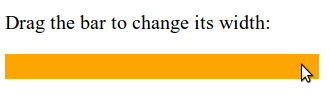
\includegraphics[width=5.3cm]{img/drag-bar.png}
\vskip 1.5ex\index{mouseup event}\index{mousemove event}

Note that the \lstinline`"mousemove"` handler is registered on the whole \index{window}window. Even if the mouse goes outside of the bar during resizing, as long as the button is held we still want to update its size.\index{buttons property}\index{button property}\index{bitfield}

We must stop resizing the bar when the mouse button is released. For that, we can use the \lstinline`buttons` property (note the plural), which tells us about the buttons that are currently held down. When this is zero, no buttons are down. When buttons are held, its value is the sum of the codes for those buttons—the left button has code 1, the right button 2, and the middle one 4. That way, you can check whether a given button is pressed by taking the remainder of the value of \lstinline`buttons` and its code.

Note that the order of these codes is different from the one used by \lstinline`button`, where the middle button came before the right one. As mentioned, consistency isn't really a strong point of the browser's programming interface.

\subsection{Touch events}\index{touch}\index{mousedown event}\index{mouseup event}\index{click event}

The style of graphical browser that we use was designed with mouse interfaces in mind, at a time where touchscreens were rare. To make the Web ``work'' on early touchscreen phones, browsers for those devices pretended, to a certain extent, that touch events were mouse events. If you tap your screen, you'll get \lstinline`"mousedown"`, \lstinline`"mouseup"`, and \lstinline`"click"` events.

But this illusion isn't very robust. A touchscreen works differently from a mouse: it doesn't have multiple buttons, you can't track the finger when it isn't on the screen (to simulate \lstinline`"mousemove"`), and it allows multiple fingers to be on the screen at the same time.

Mouse events cover touch interaction only in straightforward cases—if you add a \lstinline`"click"` handler to a button, touch users will still be able to use it. But something like the resizeable bar in the previous example does not work on a touchscreen.\index{touchstart event}\index{touchmove event}\index{touchend event}

There are specific event types fired by touch interaction. When a finger starts touching the screen, you get a \lstinline`"touchstart"` event. When it is moved while touching, \lstinline`"touchmove"` events fire. Finally, when it stops touching the screen, you'll see a \lstinline`"touchend"` event.\index{touches property}\index{clientX property}\index{clientY property}\index{pageX property}\index{pageY property}

Because many touchscreens can detect multiple fingers at the same time, these events don't have a single set of coordinates associated with them. Rather, their \index{event object}event objects have a \lstinline`touches` property, which holds an \index{array-like object}array-like object of points, each of which has its own \lstinline`clientX`, \lstinline`clientY`, \lstinline`pageX`, and \lstinline`pageY` properties.

You could do something like this to show red circles around every touching finger:

\begin{lstlisting}
<style>
  dot { position: absolute; display: block;
        border: 2px solid red; border-radius: 50px;
        height: 100px; width: 100px; }
</style>
<p>Touch this page</p>
<script>
  function update(event) {
    for (let dot; dot = document.querySelector("dot");) {
      dot.remove();
    }
    for (let i = 0; i < event.touches.length; i++) {
      let {pageX, pageY} = event.touches[i];
      let dot = document.createElement("dot");
      dot.style.left = (pageX - 50) + "px";
      dot.style.top = (pageY - 50) + "px";
      document.body.appendChild(dot);
    }
  }
  window.addEventListener("touchstart", update);
  window.addEventListener("touchmove", update);
  window.addEventListener("touchend", update);
</script>
\end{lstlisting}
\noindent\index{preventDefault method}

You'll often want to call \lstinline`preventDefault` in touch event handlers to override the browser's default behavior (which may include scrolling the page on swiping) and to prevent the mouse events from being fired, for which you may \emph{also} have a handler.

\section{Scroll events}\index{scrolling}\index{scroll event}\index{event handling}

Whenever an element is scrolled, a \lstinline`"scroll"` event is fired on it. This has various uses, such as knowing what the user is currently looking at (for disabling off-screen \index{animation}animations or sending \index{spy}spy reports to your evil headquarters) or showing some indication of progress (by highlighting part of a table of contents or showing a page number).

The following example draws a \index{progress bar}progress bar above the document and updates it to fill up as you scroll down:

\begin{lstlisting}
<style>
  #progress {
    border-bottom: 2px solid blue;
    width: 0;
    position: fixed;
    top: 0; left: 0;
  }
</style>
<div id="progress"></div>
<script>
  // Create some content
  document.body.appendChild(document.createTextNode(
    "supercalifragilisticexpialidocious ".repeat(1000)));

  let bar = document.querySelector("#progress");
  window.addEventListener("scroll", () => {
    let max = document.body.scrollHeight - innerHeight;
    bar.style.width = `${(pageYOffset / max) * 100}%`;
  });
</script>
\end{lstlisting}
\noindent\index{unit (CSS)}\index{scrolling}\index{position (CSS)}\index{fixed positioning}\index{absolute positioning}\index{percentage}\index{repeat method}

Giving an element a \lstinline`position` of \lstinline`fixed` acts much like an \lstinline`absolute` position but also prevents it from scrolling along with the rest of the document. The effect is to make our progress bar stay at the top. Its width is changed to indicate the current progress. We use \lstinline`%`, rather than \lstinline`px`, as a unit when setting the width so that the element is sized relative to the page width.\index{innerHeight property}\index{innerWidth property}\index{pageYOffset property}

The global \lstinline`innerHeight` binding gives us the height of the window, which we have to subtract from the total scrollable height—you can't keep scrolling when you hit the bottom of the document. There's also an \lstinline`innerWidth` for the window width. By dividing \lstinline`pageYOffset`, the current scroll position, by the maximum scroll position and multiplying by 100, we get the percentage for the progress bar.\index{preventDefault method}

Calling \lstinline`preventDefault` on a scroll event does not prevent the scrolling from happening. In fact, the event handler is called only \emph{after} the scrolling takes place.

\section{Focus events}\index{event handling}\index{focus event}\index{blur event}

When an element gains \index{focus}focus, the browser fires a \lstinline`"focus"` event on it. When it loses focus, the element gets a \lstinline`"blur"` event.\index{event propagation}

Unlike the events discussed earlier, these two events do not propagate. A handler on a parent element is not notified when a child element gains or loses focus.\index{input (HTML tag)}\index{help text example}

The following example displays help text for the \index{text field}text field that currently has focus:

\begin{lstlisting}
<p>Name: <input type="text" data-help="Your full name"></p>
<p>Age: <input type="text" data-help="Your age in years"></p>
<p id="help"></p>

<script>
  let help = document.querySelector("#help");
  let fields = document.querySelectorAll("input");
  for (let field of Array.from(fields)) {
    field.addEventListener("focus", event => {
      let text = event.target.getAttribute("data-help");
      help.textContent = text;
    });
    field.addEventListener("blur", event => {
      help.textContent = "";
    });
  }
</script>
\end{lstlisting}
\noindent

This screenshot shows the help text for the age field.

\vskip 1.5ex
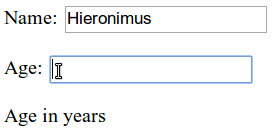
\includegraphics[width=4.4cm]{img/help-field.png}
\vskip 1.5ex\index{focus event}\index{blur event}

The \index{window}window object will receive \lstinline`"focus"` and \lstinline`"blur"` events when the user moves from or to the browser tab or window in which the document is shown.

\section{Load event}\index{script (HTML tag)}\index{load event}

When a page finishes loading, the \lstinline`"load"` event fires on the window and the document body objects. This is often used to schedule \index{initialization}initialization actions that require the whole \index{document}document to have been built. Remember that the content of \lstinline`<script>` tags is run immediately when the tag is encountered. This may be too soon, for example when the script needs to do something with parts of the document that appear after the \lstinline`<script>` tag.\index{event propagation}\index{img (HTML tag)}

Elements such as \index{image}images and script tags that load an external file also have a \lstinline`"load"` event that indicates the files they reference were loaded. Like the focus-related events, loading events do not propagate.\index{beforeunload event}\index{page reload}\index{preventDefault method}

When a page is closed or navigated away from (for example, by following a link), a \lstinline`"beforeunload"` event fires. The main use of this event is to prevent the user from accidentally losing work by closing a document. If you prevent the default behavior on this event \emph{and} set the \lstinline`returnValue` property on the event event object to a string, the browser will show the user a dialog asking if they really want to leave the page. That dialog might include your string, but because some malicious sites try to use these dialogs to confuse people into staying on their page to look at dodgy weight loss ads, most browsers no longer display them.

\label{event.timeline}\section{Events and the event loop}\index{requestAnimationFrame function}\index{event handling}\index{timeline}\index{script (HTML tag)}

In the context of the event loop, as discussed in \hyperref[async]{Chapter 11}, browser event handlers behave like other asynchronous notifications. They are scheduled when the event occurs but must wait for other scripts that are running to finish before they get a chance to run.

The fact that events can be processed only when nothing else is running means that, if the event loop is tied up with other work, any interaction with the page (which happens through events) will be delayed until there's time to process it. So if you schedule too much work, either with long-running event handlers or with lots of short-running ones, the page will become slow and cumbersome to use.

For cases where you \emph{really} do want to do some time-consuming thing in the background without freezing the page, browsers provide something called \emph{\index{web worker}web workers}. A worker is a JavaScript process that runs alongside the main script, on its own timeline.

Imagine that squaring a number is a heavy, long-running computation that we want to perform in a separate \index{thread}thread. We could write a file called \lstinline`code/squareworker.js` that responds to messages by computing a square and sending a message back.

\begin{lstlisting}
addEventListener("message", event => {
  postMessage(event.data * event.data);
});
\end{lstlisting}
\noindent

To avoid the problems of having multiple \index{thread}threads touching the same data, workers do not share their \index{global scope}global scope or any other data with the main script's environment. Instead, you have to communicate with them by sending messages back and forth.

This code spawns a worker running that script, sends it a few messages, and outputs the responses.

\begin{lstlisting}
let squareWorker = new Worker("code/squareworker.js");
squareWorker.addEventListener("message", event => {
  console.log("The worker responded:", event.data);
});
squareWorker.postMessage(10);
squareWorker.postMessage(24);
\end{lstlisting}
\noindent\index{postMessage method}\index{message event}

The \lstinline`postMessage` function sends a message, which will cause a \lstinline`"message"` event to fire in the receiver. The script that created the worker sends and receives messages through the \lstinline`Worker` object, whereas the worker talks to the script that created it by sending and listening directly on its \index{global scope}global scope. Only values that can be represented as JSON can be sent as messages—the other side will receive a \emph{copy} of them, rather than the value itself.

\section{Timers}\index{timeout}\index{setTimeout function}

We saw the \lstinline`setTimeout` function in \hyperref[async]{Chapter 11}. It schedules another function to be called later, after a given number of milliseconds.\index{clearTimeout function}

Sometimes you need to cancel a function you have scheduled. This is done by storing the value returned by \lstinline`setTimeout` and calling \lstinline`clearTimeout` on it.

\begin{lstlisting}
let bombTimer = setTimeout(() => {
  console.log("BOOM!");
}, 500);

if (Math.random() < 0.5) { // 50% chance
  console.log("Defused.");
  clearTimeout(bombTimer);
}
\end{lstlisting}
\noindent\index{cancelAnimationFrame function}\index{requestAnimationFrame function}

The \lstinline`cancelAnimationFrame` function works in the same way as \lstinline`clearTimeout`—calling it on a value returned by \lstinline`requestAnimationFrame` will cancel that frame (assuming it hasn't already been called).\index{setInterval function}\index{clearInterval function}\index{repetition}

A similar set of functions, \lstinline`setInterval` and \lstinline`clearInterval`, are used to set timers that should \emph{repeat} every \emph{X} milliseconds.

\begin{lstlisting}
let ticks = 0;
let clock = setInterval(() => {
  console.log("tick", ticks++);
  if (ticks == 10) {
    clearInterval(clock);
    console.log("stop.");
  }
}, 200);
\end{lstlisting}
\noindent

\section{Debouncing}\index{optimization}\index{mousemove event}\index{scroll event}\index{blocking}

Some types of events have the potential to fire rapidly, many times in a row (the \lstinline`"mousemove"` and \lstinline`"scroll"` events, for example). When handling such events, you must be careful not to do anything too time-consuming or your handler will take up so much time that interaction with the document starts to feel slow.\index{setTimeout function}

If you do need to do something nontrivial in such a handler, you can use \lstinline`setTimeout` to make sure you are not doing it too often. This is usually called \emph{\index{debouncing}debouncing} the event. There are several slightly different approaches to this.\index{textarea (HTML tag)}\index{clearTimeout function}\index{keydown event}

In the first example, we want to react when the user has typed something, but we don't want to do it immediately for every input event. When they are \index{typing}typing quickly, we just want to wait until a pause occurs. Instead of immediately performing an action in the event handler, we set a timeout. We also clear the previous timeout (if any) so that when events occur close together (closer than our timeout delay), the timeout from the previous event will be canceled.

\begin{lstlisting}
<textarea>Type something here...</textarea>
<script>
  let textarea = document.querySelector("textarea");
  let timeout;
  textarea.addEventListener("input", () => {
    clearTimeout(timeout);
    timeout = setTimeout(() => console.log("Typed!"), 500);
  });
</script>
\end{lstlisting}
\noindent\index{sloppy programming}

Giving an undefined value to \lstinline`clearTimeout` or calling it on a timeout that has already fired has no effect. Thus, we don't have to be careful about when to call it, and we simply do so for every event.\index{mousemove event}

We can use a slightly different pattern if we want to space responses so that they're separated by at least a certain length of \index{time}time but want to fire them \emph{during} a series of events, not just afterward. For example, we might want to respond to \lstinline`"mousemove"` events by showing the current coordinates of the mouse but only every 250 milliseconds.

\begin{lstlisting}
<script>
  let scheduled = null;
  window.addEventListener("mousemove", event => {
    if (!scheduled) {
      setTimeout(() => {
        document.body.textContent =
          `Mouse at ${scheduled.pageX}, ${scheduled.pageY}`;
        scheduled = null;
      }, 250);
    }
    scheduled = event;
  });
</script>
\end{lstlisting}
\noindent

\section{Summary}

Event handlers make it possible to detect and react to events happening in our web page. The \lstinline`addEventListener` method is used to register such a handler.

Each event has a type (\lstinline`"keydown"`, \lstinline`"focus"`, and so on) that identifies it. Most events are called on a specific DOM element and then \emph{propagate} to that element's ancestors, allowing handlers associated with those elements to handle them.

When an event handler is called, it is passed an event object with additional information about the event. This object also has methods that allow us to stop further propagation (\lstinline`stopPropagation`) and prevent the browser's default handling of the event (\lstinline`preventDefault`).

Pressing a key fires \lstinline`"keydown"` and \lstinline`"keyup"` events. Pressing a mouse button fires \lstinline`"mousedown"`, \lstinline`"mouseup"`, and \lstinline`"click"` events. Moving the mouse fires \lstinline`"mousemove"` events. Touchscreen interaction will result in \lstinline`"touchstart"`, \lstinline`"touchmove"`, and \lstinline`"touchend"` events.

Scrolling can be detected with the \lstinline`"scroll"` event, and focus changes can be detected with the \lstinline`"focus"` and \lstinline`"blur"` events. When the document finishes loading, a \lstinline`"load"` event fires on the window.

\section{Exercises}

\subsection{Balloon}\index{balloon (exercise)}\index{arrow key}

Write a page that displays a \index{balloon}balloon (using the balloon \index{emoji}emoji, 🎈). When you press the up arrow, it should inflate (grow) 10 percent, and when you press the down arrow, it should deflate (shrink) 10 percent.\index{font-size (CSS)}

You can control the size of text (emoji are text) by setting the \lstinline`font-size` CSS property (\lstinline`style.fontSize`) on its parent element. Remember to include a unit in the value—for example, pixels (\lstinline`10px`).

The key names of the arrow keys are \lstinline`"ArrowUp"` and \lstinline`"ArrowDown"`. Make sure the keys change only the balloon, without scrolling the page.

When that works, add a feature where, if you blow up the balloon past a certain size, it explodes. In this case, exploding means that it is replaced with an 💥 emoji, and the event handler is removed (so that you can't inflate or deflate the explosion).

\subsection{Mouse trail}\index{animation}\index{mouse trail (exercise)}

In JavaScript's early days, which was the high time of \index{gaudy home
pages}gaudy home
pages with lots of animated images, people came up with some truly inspiring ways to use the language.

One of these was the \emph{mouse trail}—a series of elements that would follow the mouse pointer as you moved it across the page.\index{absolute positioning}\index{background (CSS)}

In this exercise, I want you to implement a mouse trail. Use absolutely positioned \lstinline`<div>` elements with a fixed size and background color (refer to the \hyperref[event.mouse_drawing]{code} in the ``Mouse Clicks'' section for an example). Create a bunch of such elements and, when the mouse moves, display them in the wake of the mouse pointer.\index{mousemove event}

There are various possible approaches here. You can make your solution as simple or as complex as you want. A simple solution to start with is to keep a fixed number of trail elements and cycle through them, moving the next one to the mouse's current position every time a \lstinline`"mousemove"` event occurs.

\subsection{Tabs}\index{tabbed interface (exercise)}

Tabbed panels are widely used in user interfaces. They allow you to select an interface panel by choosing from a number of tabs ``sticking out'' above an element.\index{button (HTML tag)}\index{display (CSS)}\index{hidden element}\index{data attribute}

In this exercise you must implement a simple tabbed interface. Write a function, \lstinline`asTabs`, that takes a DOM node and creates a tabbed interface showing the child elements of that node. It should insert a list of \lstinline`<button>` elements at the top of the node, one for each child element, containing text retrieved from the \lstinline`data-tabname` attribute of the child. All but one of the original children should be hidden (given a \lstinline`display` style of \lstinline`none`). The currently visible node can be selected by clicking the buttons.

When that works, extend it to style the button for the currently selected tab differently so that it is obvious which tab is selected.
